\chapter{Getting Started}\label{bootup}

\begin{fortune}
This login session: \$13.99, but for you \$11.88.
\end{fortune}

You may have previous experience with MS-DOS\index{MS-DOS} or other
single user operating systems, such as OS/2\index{OS/2} or the
Macintosh.\index{Macintosh}  In these operating systems, you didn't
have to identify yourself to the computer before using it; it was
assumed that you were the only user of the system and could access
everything. Well, \unix\ is a multi-user operating system---not only
can more than one person use it at a time, different people are
treated differently.

To tell people apart, \unix\ needs a user to identify him or
herself\footnote{From here on in this book, I shall be using the
masculine pronouns to identify all people.  This is the standard
English convention, and people shouldn't take it as a statement that
only men can use computers.} by a process called \concept{logging in}.
When you first turn on the computer a complex process takes place
before the computer is ready for someone to use it.
Since this guide is geared towards \linux,
I'll tell you what happens during the \linux\ boot-up
sequence.\glossary{boot-up}

If you're using \linux\ on some type of computer besides an
Intel\index{Intel} PC, some things in this chapter won't apply to you.
Mostly, they'll be in Section~\ref{intel-powerup}.

If you're just interested in using your computer, you can skip all the
information in the chapter except for
Section~\ref{actual-login-section}.

\section{Power to the Computer}\label{intel-powerup}

The first thing that happens when you turn an Intel\index{Intel} PC on
is that the BIOS\index{BIOS}\glossary{BIOS} executes. BIOS\index{BIOS}
stands for {\bf B}asic {\bf I}nput/{\bf O}utput {\bf S}ystem.  It's a
program permenantly stored in the computer on read-only chips.  It
performs some minimal tests, and then looks for a floppy disk in the
first disk drive.  If it finds one, it looks for a ``boot sector'' on
that disk, and starts executing code from it, if any.  If there is a
disk, but no boot sector, the BIOS will print a message like:
\begin{screen}\begin{verbatim}
Non-system disk or disk error
\end{verbatim}\end{screen}
Removing the disk and pressing a key will cause the boot process to
continue.

If there isn't a floppy disk in the drive, the BIOS\index{BIOS} looks
for a master boot record\glossary{master boot record}
\index{master boot record} (MBR) on the hard disk.  It will start
executing the code found there, which loads the operating system.  On
\linux\ systems, LILO\index{LILO}, the {\bf LI}nux {\bf LO}ader, can
occupy the MBR position, and will load \linux.  For now, we'll assume
that happens and that \linux\ starts to load. (Your particular
distribution may handle booting from the hard disk differently.  Check
with the documentation included with the distribution. Another good
reference is the LILO\index{LILO} documentation,~\cite{Al:LILO}.)

\section{\linux\ Takes Over}\label{linux-powerup}

After the BIOS\index{BIOS} passes control to LILO\index{LILO}, LILO
passes control to the \linux\ \concept{kernel}.  A kernel is the
central program of the operating system, in control of all other
programs.  The first thing that \linux\ does once it starts executing
is to change to protected mode.\glossary{protected mode} The
80386\footnote{When I refer to the 80386, I am also talking about the
  80486, Pentium, and Pentium Pro computers unless I specifically say
  so.  Also, I'll be abbreviating 80386 as 386.} CPU that controls
your computer has two modes called ``real mode''\glossary{real mode}
and ``protected mode''.  DOS\index{DOS} runs in real mode, as does the
BIOS.\index{BIOS} However, for more advanced operating systems, it is
necessary to run in protected mode.  Therefore, when \linux\ boots, it
discardes the BIOS.

Other CPUs will get to this stage differently.  No other CPU needs to
switch into protected mode and few have to have such a heavy framework
around the loading procedure as LILO and the BIOS.  Once the kernel
starts up, \linux\ works much the same.

\begin{figure}[tb]\label{bootup-figure}
\centering
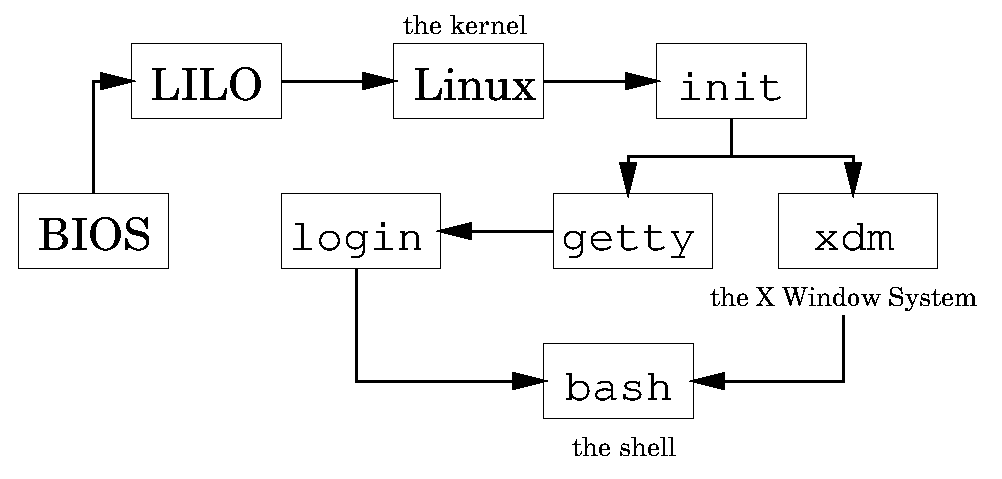
\epsfig{file=ps-files/bootup-figure.ps, width=.9\linewidth}
\caption{The path an Intel PC takes to get to a shell prompt. {\tt
    init} may or may not start the X Window System.  If it does, {\tt
    xdm} runs.  Otherwise, {\tt getty} runs.}
\end{figure}

\linux\ then looks at the type of hardware it's running on.  It wants
to know what type of hard disks you have, whether or not you have a
bus mouse, whether or not you're on a network, and other bits of
trivia like that.  \linux\ can't remember things between boots, so it
has to ask these questions each time it starts up.  Luckily, it isn't
asking {\em you\/} these questions---it is asking the hardware!
During boot-up, the \linux\ kernel will print variations on several
messages. You can read about the messages in
Section~\ref{kernel-messages}.  This query process can some cause
problems with your system but if it was going to, it probably would
have when you first installed \linux.  If you're having problems,
consult your distribution's documentation.

The kernel merely manages other programs, so once it is satisfied
everything is okay, it must start another program to do anything
useful. The program the kernel starts is called {\tt init}
\ttindex{init}.  (Notice the difference in font.  Things in {\tt this
  font} are usually the names of programs, files, directories, or
other computer related items.) After the kernel starts {\tt
  init}\ttindex{init}, it never starts another program. The kernel
becomes a manager and a provider, not an active program.

So to see what the computer is doing after the kernel boots up, we'll
have to examine {\tt init}\ttindex{init}. {\tt init}\ttindex{init}
goes through a complicated startup sequence that isn't the same for
all computers.  \linux\ has many different versions of {\tt
  init}\ttindex{init}, and each does things its own way. It also
matters whether your computer is on a network and what distribution
you used to install \linux. Some things that might happen once {\tt
  init}\ttindex{init} is started:

\begin{itemize}
\item The file systems\glossary{file system} might be checked. What is
  a file system?  A file system is the layout of files on the hard
  disk.  It let's \linux\ know which parts of the disk are already
  used, and which aren't.  (It's like an index to a rather large
  filing system or a card catalog to a library.)  Unfortunately, due
  to various factors such as power losses, what the file system
  information thinks is going on in the rest of the disk and the
  actually layout of the rest of the disk are occasionally in
  conflict. A special program, called {\tt fsck}, can find these
  situations and hopefully correct them.

\item Special routing\glossary{route} programs for
  networks\glossary{network} are run.  These programs tell your
  computer how it's suppose to contact other computers.

\item Temporary files left by some programs may be deleted.

\item The system clock can be correctly updated.  This is trickier
  then one might think, since \unix, by default, wants the time in UCT
  (Universal Coordinated Time, also known as Greenwich Mean Time) and
  your CMOS clock, a battery powered clock in your computer, is
  probably set on local time.  This means that some program must read
  the time from your hardware clock and correct it to UCT.
\end{itemize}

After {\tt init}\ttindex{init} is finished with its duties at boot-up,
it goes on to its regularly scheduled activities. {{\tt init}}
\ttindex{init} can be called the parent of all processes
\index{process}\glossary{process} on a \unix\ system.  A process is
simply a running program.  Since one program can be running two or
more times, there can be two or more processes for any particular
program.

In \unix, a process\index{process}, an instance of a program, is
created by a system call\glossary{system call}---a service provided by
the kernel---called fork\index{process!forking}.  (It's called
``fork'' since one process splits off into two seperate ones.)  {\tt
  init}\ttindex{init} forks a couple of processes, which in turn fork
some of their own. On your \linux\ system, what {\tt init} runs are
several instances of a program called {\tt getty}.\ttindex{getty} {\tt
  getty} is the program that will allow a user to login and eventually
calls a program called {\tt login}\ttindex{login}.

\section{The User Acts}\label{actual-login-section}

\subsection{Logging In}

The first thing you have to do to use a \unix\ machine is to identify
yourself.  The \concept{login} is \unix's way of knowing that users
are authorized to use the system.  It asks for an account
name\index{account} and password.\index{password} An account name is
normally similar to your regular name; you should have already
received one from your system administrator, or created your own if
you are the system administrator. (Information on doing this should be
available in \ldpgs\ or \ldpsa.)

You should see, after all the boot-up procedures are done, something
like the following (the first line is merely a greeting message---it
might be a disclaimer or anything else):

\begin{screen}\begin{verbatim}
Welcome to the mousehouse. Please, have some cheese.

mousehouse login:
\end{verbatim}\end{screen}

\xwarn However, it's possible that what the system presents you
with does {\em not\/} look like this. Instead of a boring text mode
screen, it is graphical. However, it will still ask you to login, and
will function mostly the same way.  If this is the case on your
system, you are going to be using The X Window System\index{X Window
  System}.  This means that you will be presented with a windowing
system.  Chapter~\ref{x-chapter} will discuss some of the differences
that you'll be facing.  Logging in will be similar as will the basics
to much of \unix. If you are using X, look for a giant X is the
margin.

This is, of course, your invitation to login.\index{login} Throughout
this manual, we'll be using the fictional (or not so fictional,
depending on your machine) user {\tt larry}.  Whenever you see {\tt
  larry}, you should be substituting your own account name.  Account
names are usually based on real names; bigger, more serious \unix\ 
systems will have accounts using the user's last name, or some
combination of first and last name, or even some numbers. Possible
accounts for Larry Greenfield might be: {\tt larry}, {\tt greenfie},
{\tt lgreenfi}, {\tt lg19}.

{\tt mousehouse} is, by the way, the ``name'' of the machine I'm
working on. It is possible that when you installed \linux, you were
prompted for some very witty name. It isn't very important, but
whenever it comes up, I'll be using {\tt mousehouse} or, rarely, {\tt
lionsden} when I need to use a second system for clarity or contrast.

After entering {\tt larry} and pressing \ret, I'm faced with the
following:

\begin{screen}\begin{verbatim}
mousehouse login: larry
Password:
\end{verbatim}\end{screen}

What \linux\ is asking for is your \concept{password}. When you type
in your password, you won't be able to see what you type. Type
carefully: it is possible to delete, but you won't be able to see what
you are editing. Don't type too slowly if people are
watching---they'll be able to learn your password.  If you mistype,
you'll be presented with another chance to login.
\glossary{password}\index{password}

If you've typed your login name and password correctly, a short
message will appear, called the message of the day.  
\ttindex{/etc/motd} This could say anything---the system adminstrator
decides what it should be.  After that, a {\bf prompt}
appears.\index{shell!prompt} A prompt is just that, something
prompting you for the next command to give the system. It should look
something like this:

\begin{screen}\begin{verbatim}
/home/larry#
\end{verbatim}\end{screen}

\xwarn If you've already determined you're using X, you'll
probably see a prompt like the one above in a ``window'' somewhere on
the screen. (A ``window'' is a rectangular box.)  To type into
the prompt, move the mouse cursor (it probably looks like a big ``x''
or an arrow) using the mouse into the window.

\subsection{Leaving the Computer}

\cautionpar Do not just turn off the computer! You risk losing
valuable data!

Unlike most versions of DOS\index{DOS}, it's a bad thing to just hit
the power switch when you're done using the computer.  It is also bad
to reboot the machine (with the reset button) without first taking
proper precautions.  \linux, in order to improve performance, has a
\concept{disk cache}.  This means it temporarily stores part of the
computer's permanent storage in RAM\@.\footnote{The difference between
  ``RAM'' and a hard disk is like the difference between short term
  memory and long term memory.  Shutting off the power is like giving
  the computer a knock on the head---it'll forget everything in short
  term memory.  But things saved in long term memory, the hard disk,
  will be okay.  The disk is thousands of times slower than RAM\@.}
The idea of what \linux\ thinks the disk should be and what the disk
actually contains is syncronized every 30 seconds.  In order to turn
off or reboot the computer, you'll have to go through a procedure
telling it to stop caching disk information.

If you're done with the computer, but are logged in (you've entered a
username and password), first you must logout. To do so, enter the
command {\tt logout}. All commands are sent by pressing \ret. Until
you hit return nothing will happen and you can delete what you've
done and start over.

\begin{screen}\begin{verbatim}
/home/larry# logout

Welcome to the mousehouse. Please, have some cheese.

mousehouse login:
\end{verbatim}\end{screen}

Now another user can login.

\subsection{Turning the Computer Off}

If this is a single user system, you might want to turn the computer
off when you're done with it.\footnote{To avoid possibly weakening
  some hardware components, only turn off the computer when you're
  done for the day.  Turning the computer on and off once a day is
  probably the best compromise between energy and wear \& tear on the
  system.} To do so, you'll have to log into a special account called
{\tt root}. The {\tt root} account is the system adminstrator's
account and can access any file on the system.  If you're going to
turn the computer off, get the password from the system adminstrator.
(In a single user system, that's {\em you\/}!  Make sure you know the
{\tt root} password.) Login as {\tt root}:

\begin{screen}\begin{verbatim}
mousehouse login: root
Password:
Linux version 1.3.55 (root@mousehouse) #1 Sun Jan 7 14:56:26 EST 1996
/# shutdown now
Why? end of the day

URGENT: message from the sysadmin:
System going down NOW

          ... end of the day ...

Now you can turn off the power...
\end{verbatim}\end{screen}

The command {\tt shutdown now} prepares the system to be reset or
turned off.  Wait for a message saying it is safe to and then reset or
turn off the system.  (When the system asks you
``Why?'', it is merely asking for a reason to tell other users.  Since
no one is using the system when you shut it down, you can tell it
anything you want or nothing at all.)

A quick message to the lazy: an alternative to the logout/login
approach is to use the command {\tt su}. As a normal user, from your
prompt, type {\tt su} and press \ret. It should prompt you for the
root password, and then give you root privileges. Now you can shutdown
the system with the {\tt shutdown now} command.

\section{Kernel Messages}\label{kernel-messages}

When you first start your computer, a series of messages flash across
the screen describing the hardware that is attached to your
computer.  These messages are printed by the \linux\ kernel.  In this
section, I'll attempt to describe and explain those messages.

Naturally, these messages differ from machine to machine.  I'll
describe the messages I get for my machine.  The following example
contains all of the standard messages and some specific ones.  (In
general, the machine I'm taking this from is a minimally configured
one: you won't see a lot of device specific configuration.)  This was
made with Linux version 1.3.55---one of the most recent as of this
writing.

\index{linux kernel!starting messages@\linux\ kernel!starting messages}
\begin{enumerate}
\item The first thing \linux\ does is decides what type of video card
and screen you have, so it can pick a good font size. (The smaller the
font, the more that can fit on the screen on any one time.) \linux\
may ask you if you want a special font, or it might have had a choice
compiled in.\footnote{``Compiled'' is the process by which a computer
program that a human writes gets translated into something the
computer understands.  A feature that has been ``compiled in'' has
been included in the program.}
\begin{screen}\begin{verbatim}
Console: 16 point font, 400 scans
Console: colour VGA+ 80x25, 1 virtual console (max 63)
\end{verbatim}\end{screen}
In this example, the machine owner decided he wanted the standard,
large font at compile time.\glossary{compile}\glossary{binary} Also,
note the misspelling of the word ``color.'' Linus evidently learned
the wrong version of English.\index{Torvalds, Linus!English usage}

\item The next thing the kernel will report is how fast your system
  is, as measured by ``BogoMIPS''.\index{BogoMIPS}  A ``MIP'' stands
  for a million instructions per second, and a ``BogoMIP'' is a
  ``bogus MIP'': how many times the computer can do absolutely nothing
  in one second.  (Since this loop doesn't actually do anything, the
  number is not actually a measure of how fast the system is.)
  \linux\ uses this number when it needs to wait for a hardware
  device.
\begin{screen}\begin{verbatim}
Calibrating delay loop.. ok - 33.28 BogoMIPS
\end{verbatim}\end{screen}
  
\item The \linux\ kernel also tells you a little about memory usage:
  \begin{screen}\begin{verbatim}
Memory: 23180k/24576k available (544k kernel code, 384k reserved, 468k data)
\end{verbatim}\end{screen}
This said that the machine had 24 megabytes\glossary{megabyte} of
memory.  Some of this memory was reserved for the kernel.  The rest of
it can be used by programs.  This is the temporary \concept{RAM} that
is used only for short term storage.  Your computer also has a
permanent memory called a \concept{hard disk}.  The hard disk's
contents stay around even when power is turned off.

\item Throughout the bootup procedure, \linux\ tests different parts
  of the hardware and prints messages about these tests.
\begin{screen}\begin{verbatim}
This processor honours the WP bit even when in supervisor mode. Good.
\end{verbatim}\end{screen}

  \item Now \linux\ moves onto the network
    configuration.\glossary{network} The following should be described
    in \ldpng, and is beyond the scope of this document.
\begin{screen}\begin{verbatim}
Swansea University Computer Society NET3.033 for Linux 1.3.50
IP Protocols: ICMP, UDP, TCP
\end{verbatim}\end{screen}

  \item \linux\ supports a FPU\index{FPU}, a floating point unit. This
    is a special chip (or part of a chip, in the case of a 80486DX
    CPU\glossary{floating point unit}) that performs arithmetic
    dealing with non-whole numbers. Some of these chips are bad, and
    when \linux\ tries to identify these chips, the machine
    ``crashes''.  The machine stops functioning. If this happens,
    you'll see:
\begin{screen}\begin{verbatim}
Checking 386/387 coupling...
\end{verbatim}\end{screen}\index{error!bad 386/387 coupling}
Otherwise, you'll see:
\begin{screen}\begin{verbatim}
Checking 386/387 coupling... Ok, fpu using exception 16 error reporting.
\end{verbatim}\end{screen}
if you're using a 486DX\@.  If you are using a 386 with a 387, you'll see:
\begin{screen}\begin{verbatim}
Checking 386/387 coupling... Ok, fpu using irq13 error reporting.
\end{verbatim}\end{screen}

\item It now runs another test on the ``halt'' instruction.
\begin{screen}\begin{verbatim}
Checking 'hlt' instruction... Ok.
\end{verbatim}\end{screen}
  
\item After that initial configuration, \linux\ prints a line
  identifying itself.  It says what version it is, what
  version of the GNU C Compiler compiled it, and when it was compiled.
\begin{screen}\begin{verbatim}
Linux version 1.3.55 (root@mousehouse) (gcc version 2.7.0) #1 Sun Jan 7 14:56:26 EST 1996
\end{verbatim}\end{screen}

  \item The serial \index{serial ports} driver has started to ask
    questions about the hardware.  A \concept{driver} is a part of the
    kernel that controls a device, usually a peripheral.  It is
    responsible for the details of how the CPU communicates with the
    device.  This allows people who write user applications to
    concentrate on the application: they don't have to worry about
    exactly how the computer works.
\begin{screen}\begin{verbatim}
Serial driver version 4.11 with no serial options enabled
tty00 at 0x03f8 (irq = 4) is a 16450
tty01 at 0x02f8 (irq = 3) is a 16450
tty02 at 0x03e8 (irq = 4) is a 16450
\end{verbatim}\end{screen}
Here, it found 3 serial ports.  A serial port is the equivalent of
a DOS\index{DOS} {\tt COM} port, and is a device normally used to
communicate with
modems and mice.

What it is trying to say is that serial port 0 ({\tt COM1}) has an
address of {\tt 0x03f8}. When it interrupts the kernel,
usually to say that it has data, it uses IRQ 4. An IRQ is another
means of a peripheral talking to the software.  Each serial port also
has a controller chip.  The usual one for a port to have is a 16450;
other values possible are 8250 and 16550. 

\item Next comes the parallel port driver.  A parallel port is
\index{parallel ports}
normally connected to a printer, and the names for the parallel ports
(in \linux) start with {\tt lp}. {\tt lp} stands for {\bf L}ine {\bf
P}rinter, although in modern times it makes more sense for it to stand
for {\bf L}aser {\bf P}rinter.  (However, \linux\ will happily
communicate with any sort of parallel printer: dot matrix, ink jet, or
laser.)
\begin{screen}\begin{verbatim}
lp0 at 0x03bc, (polling)
\end{verbatim}\end{screen}
That message says it has found one parallel port, and is using the
standard driver for it.

\item \linux\ next identifies your hard disk drives.  In the example
  system I'm showing you, {\tt mousehouse}, I've installed two IDE
  hard disk drives.
\begin{screen}\begin{verbatim}
hda: WDC AC2340, 325MB w/127KB Cache, CHS=1010/12/55
hdb: WDC AC2850F, 814MB w/64KB Cache, LBA, CHS=827/32/63
\end{verbatim}\end{screen}
  

\item The kernel now moves onto looking at your floppy drives. In this
example, the machine has two drives: drive ``A'' is
a $5\ {1/4}$ inch drive, and drive ``B'' is a $3\ {1/2}$ inch drive.
\linux\ calls drive ``A'' {\tt fd0} and drive ``B'' {\tt fd1}.
\begin{screen}\begin{verbatim}
Floppy drive(s): fd0 is 1.44M, fd1 is 1.2M
floppy: FDC 0 is a National Semiconductor PC87306
\end{verbatim}\end{screen}

\item The next driver to start on my example system is the SLIP
  driver.  It prints out a message about its configuration.
\begin{screen}\begin{verbatim}
SLIP: version 0.8.3-NET3.019-NEWTTY (dynamic channels, max=256) (6 bit encapsulation enabled)
CSLIP: code copyright 1989 Regents of the University of California
\end{verbatim}\end{screen}

  \item The kernel also scans the hard disks it found.  It will look
    for the different partitions on each of them.  A partition is a
    logical separation on a drive that is used to keep operating
    systems from interfering with each other. In this example, the
    computer had two hard disks ({\tt hda}, {\tt hdb}) with four
    partitions and one partition, respectively.\index{partition!disk}
\begin{screen}\begin{verbatim}
Partition check:
  hda: hda1 hda2 hda3 hda4
  hdb: hdb1
\end{verbatim}\end{screen}

\item Finally, \linux\ {\bf mounts}\glossary{mount}\index{mount} the
  root partition.  The root partition is the disk partition where the
  \linux\ operating system resides.\index{partition!root}  When
  \linux\ ``mounts'' this partition, it is making the partition
  available for use by the user.
\begin{screen}\begin{verbatim}
VFS: Mounted root (ext2 filesystem) readonly.
\end{verbatim}\end{screen}
\end{enumerate} % kernel start-up messages
% Local Variables: 
% mode: latex
% TeX-master: "guide"
% End: 
